% =====================================================================
% NaviPath-CL — "Selection Forgetting + Sequential Budgeted Observer"
% Draft v2.0 — 2026-06-30
% Template: MICCAI 2026 LNCS (adapt header for other venues).
% - Anonymized for double-blind; camera-ready: uncomment author block.
% - v2.0: adds Sequential Budgeted Observer (SBO) + MMR formulas,
%         ZeroSlide zero-shot baseline, λ sweep results, LoRA future work.
% =====================================================================
\documentclass[runningheads]{llncs}

\usepackage[T1]{fontenc}
\usepackage{graphicx}
\usepackage{amsmath,amssymb,amsthm}
\usepackage{booktabs}
\usepackage{array}
\usepackage{xcolor}
\usepackage{placeins}
\usepackage{algorithm}
\usepackage{algpseudocode}
\usepackage[hidelinks]{hyperref}
\graphicspath{{figs/}}

% ---- handy macros ----
\newcommand{\go}{\ensuremath{\checkmark}}
\newcommand{\nogo}{\ensuremath{\times}}
\newcommand{\K}{\ensuremath{K}}
\newcommand{\Stask}[1]{\mathcal{S}^{(#1)}}
\newcommand{\Sacc}[1]{\mathcal{S}^{(\leq #1)}}

% ---- float placement ----
\renewcommand{\topfraction}{0.92}
\renewcommand{\bottomfraction}{0.85}
\renewcommand{\textfraction}{0.07}
\renewcommand{\floatpagefraction}{0.82}
\setcounter{topnumber}{3}
\setcounter{bottomnumber}{2}
\setcounter{totalnumber}{4}

\begin{document}

\title{NaviPath-CL: Continual Navigation of Whole-Slide Images via
Budgeted Sequential Observation and Skill Memory}
\titlerunning{NaviPath-CL: Continual WSI Navigation}

\author{Anonymized Authors}
\authorrunning{Anonymized Author et al.}
\institute{Anonymized Affiliations \\ \email{email@anonymized.com}}

% Camera-ready (uncomment after acceptance):
% \author{Aaron Hung\inst{1} \and ...}
% \authorrunning{Hung et al.}
% \institute{...\\ \email{...}}

\maketitle

% =====================================================================
\begin{abstract}
Gigapixel whole-slide images (WSIs) contain thousands of patches, yet
practical diagnosis observes only a small \emph{budget} of patches
through a learned \textbf{observation policy}. We study an overlooked
failure mode: under a continual stream of WSI tasks, this observation
policy suffers \textbf{selection forgetting}---collapsing below a
random baseline for old tasks even when the diagnostic backbone is
fully frozen (classifier-level forgetting is zero by construction). We
propose the \textbf{Continual Navigation Layer (CNL)}, comprising:
(i)~a lightweight \textbf{MicroRouter} that learns patch importance
scores under weak supervision; (ii)~a \textbf{Sequential Budgeted
Observer (SBO)} that selects patches in adaptive, evidence-driven
rounds via Maximal Marginal Relevance (MMR) redundancy; and (iii)~a
\textbf{Navigation Skill Memory (NSM)} that stores per-task navigation
policies, recovering mACC from $0.595$ to $\mathbf{0.935}$ with zero
forgetting. A zero-shot navigation baseline (frozen FM text--patch
similarity, no training) achieves mACC $0.858$~\cite{zeroslide},
confirming that learned navigation skill provides further gains. A
$\lambda$ sweep over the SBO diversity parameter shows that optimal
$\lambda{=}0.5$--$1.0$ reflects the spatial clustering of diagnostic
regions; we propose LoRA-NSM (${\sim}130\times$ fewer parameters/task)
as the scalable next step.
\keywords{Continual learning \and Whole-slide images \and Patch
selection \and Foundation models \and Sequential observation \and
Catastrophic forgetting}
\end{abstract}

% =====================================================================
\section{Introduction}
\label{sec:intro}

Whole-slide images are gigapixel and are typically classified under
multiple-instance learning (MIL)~\cite{ilse2018abmil,lu2021clam}.
Recent pathology foundation models supply strong \textbf{frozen} patch
encoders~\cite{lu2024conch,chen2024uni}, and prompt- or
prototype-based vision--language MIL adapts them by learning only
small task descriptors while the encoder stays
frozen~\cite{gou2025qpmil}. Freezing removes the classical source of
catastrophic forgetting---the representation cannot drift. Yet a slide
contains thousands of patches, and under compute budgets a model must
decide \textbf{which patches to examine}. This \emph{observation
policy} is itself trainable, and whether it survives continual
learning has, to our knowledge, not been examined.

\noindent\textbf{Selection forgetting.} We show that a lightweight
trainable patch router, attached to a frozen diagnostic backbone,
selects well for the most-recent task but, for older tasks,
\textbf{collapses below random}---a phenomenon we term \textbf{selection
forgetting}. Because the predictor is unchanged, every degradation is
attributable to the selection module alone. A same-task recency-flip
test (identical task/data/architecture, varying only recency) drops
accuracy from ${\sim}0.9$ to $0.33$--$0.40$, even for the
sample-abundant lung task, ruling out difficulty/size confounds.

\noindent\textbf{Our solution: CNL.} We propose the \textbf{Continual
Navigation Layer (CNL)} with three components. \emph{MicroRouter}: a
${\approx}132$K-param MLP learning task-specific routing skills under
weak supervision. \emph{Sequential Budgeted Observer (SBO)}: replaces
static top-$K$ selection with adaptive multi-round selection that
penalizes redundancy via MMR~\cite{carbonell1998mmr}, making
observation genuinely sequential. \emph{Navigation Skill Memory
(NSM)}: stores per-task router snapshots; during evaluation an oracle
context gate retrieves the correct skill, recovering mACC from $0.595$
to $\mathbf{0.935}$ with Forgetting~$=0$.

\noindent\textbf{Zero-shot navigation.} We introduce a zero-shot
baseline~\cite{zeroslide} that scores patches by frozen FM text--patch
similarity (no training, mACC $0.858$), providing a strong
training-free comparison point.

\noindent\textbf{Contributions.}
\begin{enumerate}
\item We identify and formalize \textbf{selection forgetting} in
frozen-FM continual WSI classification.
\item We propose the \textbf{CNL} framework: MicroRouter + SBO + NSM
(backbone-agnostic, any frozen FM).
\item We introduce the \textbf{Sequential Budgeted Observer} with MMR
redundancy; the $\lambda$ sweep reveals that optimal diversity
respects learned spatial priors of diagnostic regions.
\item We provide a \textbf{zero-shot navigation baseline}
(ZeroSlide-inspired, training-free) as a rigorous comparison.
\item NSM recovers old-task navigation; we propose \textbf{LoRA-NSM}
(${\sim}4$KB/task) as a scalable direction.
\end{enumerate}

% =====================================================================
\section{Related Work}
\label{sec:related}

\noindent\textbf{MIL and foundation models for WSIs.}
MIL pools patch features into slide-level
predictions~\cite{ilse2018abmil,lu2021clam,shao2021transmil,li2021dsmil}.
Pathology foundation models~\cite{lu2024conch,chen2024uni,huang2023plip}
extend image--text pretraining~\cite{radford2021clip}; prompt- and
prototype-based VL MIL keeps encoders frozen, including
continually~\cite{gou2025qpmil}. These methods do not study
\emph{which patches to select under a budget across tasks}.

\noindent\textbf{Continual learning.}
Regularization~\cite{kirkpatrick2017ewc},
distillation~\cite{li2017lwf}, and
replay~\cite{rebuffi2017icarl,chaudhry2019agem,buzzega2020der}; prompt
CL~\cite{wang2022l2p,wang2022dualprompt,smith2023coda}; continual
MIL~\cite{li2025akdpmp}. We expose forgetting of the
\textbf{patch-selection mechanism} and test whether a standard
replay-free regularizer mitigates it.

\noindent\textbf{Budgeted and agentic WSI inference.}
IPS~\cite{bergner2023ips} iteratively refines patch selection.
RLogist~\cite{zhao2023rlogist} uses RL to navigate slides
across resolutions. ZeroSlide~\cite{zeroslide} proposes scoring
patches by frozen FM text--patch similarity without training, which
we adopt as our zero-shot baseline. These works operate in a
single-task setting; we add the continual-learning dimension.

\noindent\textbf{Parameter-efficient fine-tuning.}
LoRA~\cite{hu2022lora} augments frozen layers with low-rank adapters;
we identify LoRA-NSM as the path to scalable skill memory.

% =====================================================================
\section{Method}
\label{sec:method}

\begin{figure}[htbp]
\centering
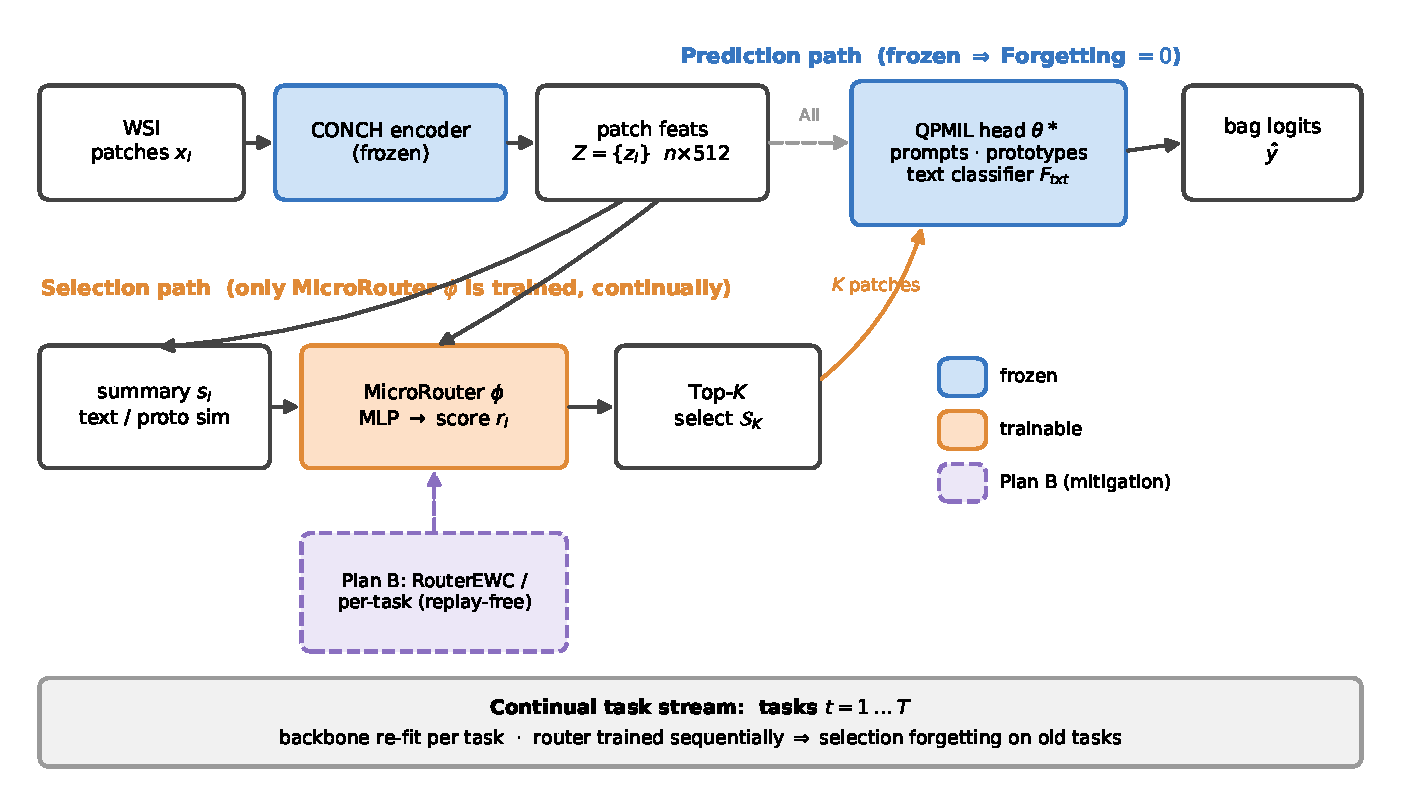
\includegraphics[width=0.68\linewidth]{Fig1_arch.pdf}
\caption{CNL's decoupled design. A frozen diagnostic backbone (blue)
shares patch features with a continually-trained MicroRouter (orange)
that scores patches; the SBO uses these scores to select patches in
adaptive rounds; NSM (purple) stores per-task router snapshots.
Because the predictor never consumes router-modified features, backbone
forgetting is zero by construction.}
\label{fig:arch}
\end{figure}

\noindent\textbf{Notation.} A slide has $n$ patches; $Z\!\in\!\mathbb{R}^{n\times D}$
are frozen foundation-encoder features ($D{=}512$, CONCH). $\hat{z}$
denotes L2-normalization. $T{=}\{t_c\}$ are class-text features;
$P{=}\{p_m\}$ are prototype features; $\phi$ is the router.

\subsection{Problem Setup}
Tasks $t{=}1,\dots,T$ arrive sequentially. After task $t$, the model
classifies slides from all tasks using $\leq K$ patches ($K\ll n$).
We decouple \emph{prediction} (frozen backbone $g_{\theta^*}$, Forgetting$\equiv0$
by construction) from \emph{navigation} (trainable router $\phi$, the
sole continually-learned component).

\subsection{Backbone Interface}
CNL interacts with any frozen diagnostic backbone via four hooks:
\texttt{encode(WSI)$\to Z$}, \texttt{class\_text\_features()$\to T$},
\texttt{prototype\_features()$\to P$},
\texttt{aggregate\_and\_predict}$(Z_\mathcal{S})$\texttt{$\to$logits}.
Instantiated here with a frozen prompt/prototype VL diagnosis
backbone~\cite{gou2025qpmil}.

\subsection{MicroRouter: Navigation Policy $\phi$}
\label{sec:router}
For each patch $i$ we compute a 4-d \textbf{task-count-invariant
summary} from frozen features:
\begin{equation}
s_i = \!\left[
  \max_c \hat{z}_i^\top \hat{t}_c,\;
  H\!\left(\operatorname{softmax}\hat{z}_i^\top \hat{T}^\top\right),\;
  \max_m \hat{z}_i^\top \hat{p}_m,\;
  \tfrac{1}{M}{\textstyle\sum}_m \hat{z}_i^\top \hat{p}_m
\right],
\label{eq:summary}
\end{equation}
then map $[z_i;s_i]\in\mathbb{R}^{516}$ through a two-layer MLP:
\begin{equation}
r_i = \underbrace{\operatorname{Linear}(256\!\to\!1)}_{\in\mathbb{R}}
      \circ\operatorname{GELU}\circ
      \underbrace{\operatorname{Linear}(516\!\to\!256)}_{}
      \bigl([z_i;s_i]\bigr).
\label{eq:router}
\end{equation}
$r_i\in\mathbb{R}$ is the patch importance score; $\phi\approx132$K
params; the router is the \textbf{only component trained across tasks}.

\noindent\textbf{Soft-route training.} Hard top-$K$ is
non-differentiable; we select $\mathcal{S}_K{=}\operatorname{top-}K_i r_i$,
softmax-weight the scores within $\mathcal{S}_K$, aggregate the bag
embedding, and compute the cross-entropy against the frozen text
classifier:
\begin{equation}
w_i{=}\frac{\exp(r_i)}{\sum_{j\in\mathcal{S}_K}\!\exp(r_j)},\quad
\bar{z}{=}\widehat{\textstyle\sum_{i\in\mathcal{S}_K}\!w_i z_i},\quad
\mathcal{L}_\text{route}{=}\operatorname{CE}\!\bigl(\sigma\bar{z}T^\top,y\bigr).
\label{eq:softroute}
\end{equation}
Gradients reach $\phi$ only through $w_i$; backbone frozen throughout.

\subsection{Zero-Shot Navigation Baseline}
\label{sec:zeroshot}
Inspired by ZeroSlide~\cite{zeroslide}, we define a training-free
navigation score using only frozen FM text--patch similarity:
\begin{equation}
r_i^{zs} = \max_c\,\hat{z}_i^\top\hat{t}_c.
\label{eq:zeroshot}
\end{equation}
No training, no task-specific parameters ($0$ bytes/task). We evaluate
it in both one-shot (\texttt{zeroshot\_oneshot}) and SBO
(\texttt{zeroshot\_seq}) modes.

\subsection{Sequential Budgeted Observer (SBO)}
\label{sec:sbo}
Static top-$K$ selection is \textbf{order-invariant}: dividing budget
$K$ into rounds yields the same patches as selecting all at once. The
SBO makes selection genuinely sequential by penalizing redundancy at
each round.

\noindent\textbf{Base score normalization.}
Router scores have task-dependent scale; we z-score-normalize them to
ensure the redundancy penalty operates at comparable scale (z-score is
monotone, so one-shot top-$K$ is unchanged):
\begin{equation}
\tilde{r}_i = \frac{r_i - \mu_r}{\sigma_r + \varepsilon},\qquad
\mu_r{=}\tfrac{1}{n}{\textstyle\sum}_i r_i,\quad
\sigma_r{=}\!\sqrt{\tfrac{1}{n}{\textstyle\sum}_i(r_i{-}\mu_r)^2}.
\label{eq:normalize}
\end{equation}

\noindent\textbf{MMR adjusted score.}
At round $t$, penalize patches similar to any already-seen patch using
Maximal Marginal Relevance~\cite{carbonell1998mmr}:
\begin{equation}
a_i^{(t)} = \tilde{r}_i - \lambda\cdot\underbrace{\max_{j\in\Sacc{t-1}}\cos(z_i,z_j)}_{\bar{m}_i^{(t)}},
\qquad a_i^{(t)}{=}{-\infty}\;\text{if }i\in\Sacc{t-1}.
\label{eq:mmr}
\end{equation}
$\lambda\geq0$ is the \textbf{diversity rotor}: $\lambda{=}0$ degrades
to static top-$K$; $\lambda{>}0$ drives the agent to new regions.

\noindent\textbf{Incremental MMR update.} After selecting $\Stask{t}$:
\begin{equation}
\bar{m}_i^{(t+1)} = \max\!\left(\bar{m}_i^{(t)},\;
\max_{j\in\Stask{t}}\cos(z_i,z_j)\right),
\label{eq:mmrupdate}
\end{equation}
achieving $O(n\cdot k_\text{step})$ per round instead of $O(n\cdot|\mathcal{S}|)$.

\noindent\textbf{Round selection.}
\begin{equation}
\Stask{t}=\operatorname{top-}k_\text{step}\!\left\{a_i^{(t)}:i\notin\Sacc{t-1}\right\}.
\label{eq:round}
\end{equation}

\noindent\textbf{Confidence-based early stopping (Route~B).}
\begin{equation}
P^{(t)}\!=\!\max_c\operatorname{softmax}\!\bigl(g_{\theta^*}(Z_{\Sacc{t}})\bigr)\geq\tau
\;\Rightarrow\;\text{stop.}
\label{eq:earlystop}
\end{equation}
When $\tau{=}\infty$, the backbone is called only once at the end
(inference cost $\approx$ one-shot).

\subsection{Navigation Skill Memory (NSM)}
\label{sec:nsm}
After training the router on task $t$, NSM stores a snapshot:
$\text{NSM}{=}\{\phi^{(1)},\dots,\phi^{(T)}\}$.
An \textbf{oracle context gate} retrieves $\phi^{(t^*)}$ for the
correct task. NSM stores \emph{routing keys} (which frozen-FM features
correlate with diagnostic relevance), not raw patch features or labels.
Storage: $\approx533$\,KB/task; 4 tasks $\approx2.1$\,MB. NSM is
an oracle upper bound; scalable LoRA-NSM is future work (Sec.~\ref{sec:lora}).

\subsection{Router Consolidation Baselines}
\label{sec:consolidation}
\noindent\textbf{Naive continual}: single router, fine-tuned
sequentially (mACC $0.595$, Forgetting $0.454$).
\noindent\textbf{EWC-on-router}: Fisher-diagonal weight regularization
on $\phi$:
\begin{equation}
F^{(t)}_j{=}\mathbb{E}_{\mathcal{D}_t}\!\bigl[(\partial\mathcal{L}_\text{route}/\partial\phi_j)^2\bigr],\;
\mathcal{L}^{(t+1)}{=}\mathcal{L}_\text{route}
{+}\lambda_\text{EWC}\!\!\sum_{\tau\leq t}\!\sum_j F^{(\tau)}_j(\phi_j{-}\phi^{*(\tau)}_j)^2.
\label{eq:ewc}
\end{equation}
\noindent\textbf{Zero-shot navigator}: $r_i^{zs}$ (Eq.~\ref{eq:zeroshot}),
training-free.
\noindent\textbf{NSM (ours)}: per-task snapshot with oracle gate.

% =====================================================================
\section{Experiments}
\label{sec:exp}

\subsection{Experimental Setup}
\textbf{Data.} Four TCGA binary subtyping tasks---esca (ESCA), rcc
(RCC subtypes), brca (BRCA), lung (NSCLC)---sequentially learned in
two orders: \textbf{reverse} (esca$\to$rcc$\to$brca$\to$lung,
smallest sample oldest) and \textbf{paper}
(lung$\to$brca$\to$rcc$\to$esca, vice versa). Three official folds;
patches encoded once by frozen CONCH ($D{=}512$)~\cite{lu2024conch}.

\noindent\textbf{Backbone.} Frozen prompt/prototype VL diagnosis
backbone~\cite{gou2025qpmil}; Adam lr~$10^{-3}$, wd~$5\!\times\!10^{-4}$,
12 epochs/task. Router: Adam lr~$5\!\times\!10^{-4}$, wd~$10^{-4}$,
5 epochs/task. Budgets $K\in\{\text{All},128,64,32,16\}$; primary
budget~$64$; SBO step size~$16$.

\subsection{Backbone Accuracy and Decoupling}
\begin{table}[htbp]
\centering
\caption{Continual accuracy (mean$\pm$std over 3 folds). Forgetting$=0$
for NaviPath is a decoupling \textbf{identity}, not a contribution.
Non-decoupled variant collapses to $0.378/0.218$ (forgetting $0.735/0.950$).}
\label{tab:acc}
\small\begin{tabular}{llccc}
\toprule
Method & Order & ACC & Forgetting & BWT \\
\midrule
VL backbone baseline & paper   & $0.924\pm0.016$ & $0.017$ & $-0.017$ \\
VL backbone baseline & reverse & $0.917\pm0.026$ & $0.041$ & $-0.041$ \\
NaviPath (CNL, ours) & paper   & $0.879\pm0.030$ & $\mathbf{0.000}$ & $0.000$ \\
NaviPath (CNL, ours) & reverse & $0.886\pm0.030$ & $\mathbf{0.000}$ & $0.000$ \\
\bottomrule
\end{tabular}
\end{table}

\subsection{Selection Forgetting: Static Router}
\begin{table}[htbp]
\centering
\caption{Router vs.\ heuristic baselines at $K{=}64$, recent vs.\ old
(accuracy, mean over 3 folds). Router is \go{} if it beats all three
heuristics; \nogo{} otherwise. Selection forgetting: recent task 6/6
GO; old task 6/6 NO-GO.}
\label{tab:router}
\small\begin{tabular}{llccccccc}
\toprule
Task & Recency & All & \textbf{Router} & Random & Proto. & Sem. & \go/\nogo \\
\midrule
esca & RECENT (paper, last)   & 0.933 & \textbf{0.956} & 0.889 & 0.711 & 0.867 & \go\,(3/3) \\
lung & RECENT (reverse, last) & 0.892 & \textbf{0.922} & 0.881 & 0.831 & 0.897 & \go\,(3/3) \\
esca & OLD (reverse, first)   & 0.867 & \textbf{0.333} & 0.822 & 0.778 & 0.778 & \nogo\,(0/3) \\
lung & OLD (paper, first)     & 0.764 & \textbf{0.397} & 0.783 & 0.705 & 0.813 & \nogo\,(0/3) \\
\bottomrule
\end{tabular}
\end{table}

\subsection{Same-Task Recency Flip: Clean Causal Test}
\label{sec:recency}

\begin{figure}[htbp]
\centering

\includegraphics[width=0.62\linewidth]{P0b_recency_flip.pdf}
\caption{\textbf{Recency flip (core result).} Same task, same test set,
same architecture; only recency differs. Accuracy flips from ${\sim}0.9$
(recent, solid) to $0.33$--$0.40$ (old, dashed), even for the
sample-abundant lung task, ruling out size/difficulty confounds.}
\label{fig:recency}
\end{figure}

For the \emph{identical} task and test set, changing only whether it
was learned last vs.\ first drops accuracy from ${\sim}0.9$ to
$0.33$--$0.40$ at $K{=}64$ (Fig.~\ref{fig:recency}). Holds for lung
(most sample-abundant), 6/6 folds, ruling out all confounds.

\subsection{Mechanism: Confident Mis-Prioritization}

\begin{figure}[htbp]
\centering
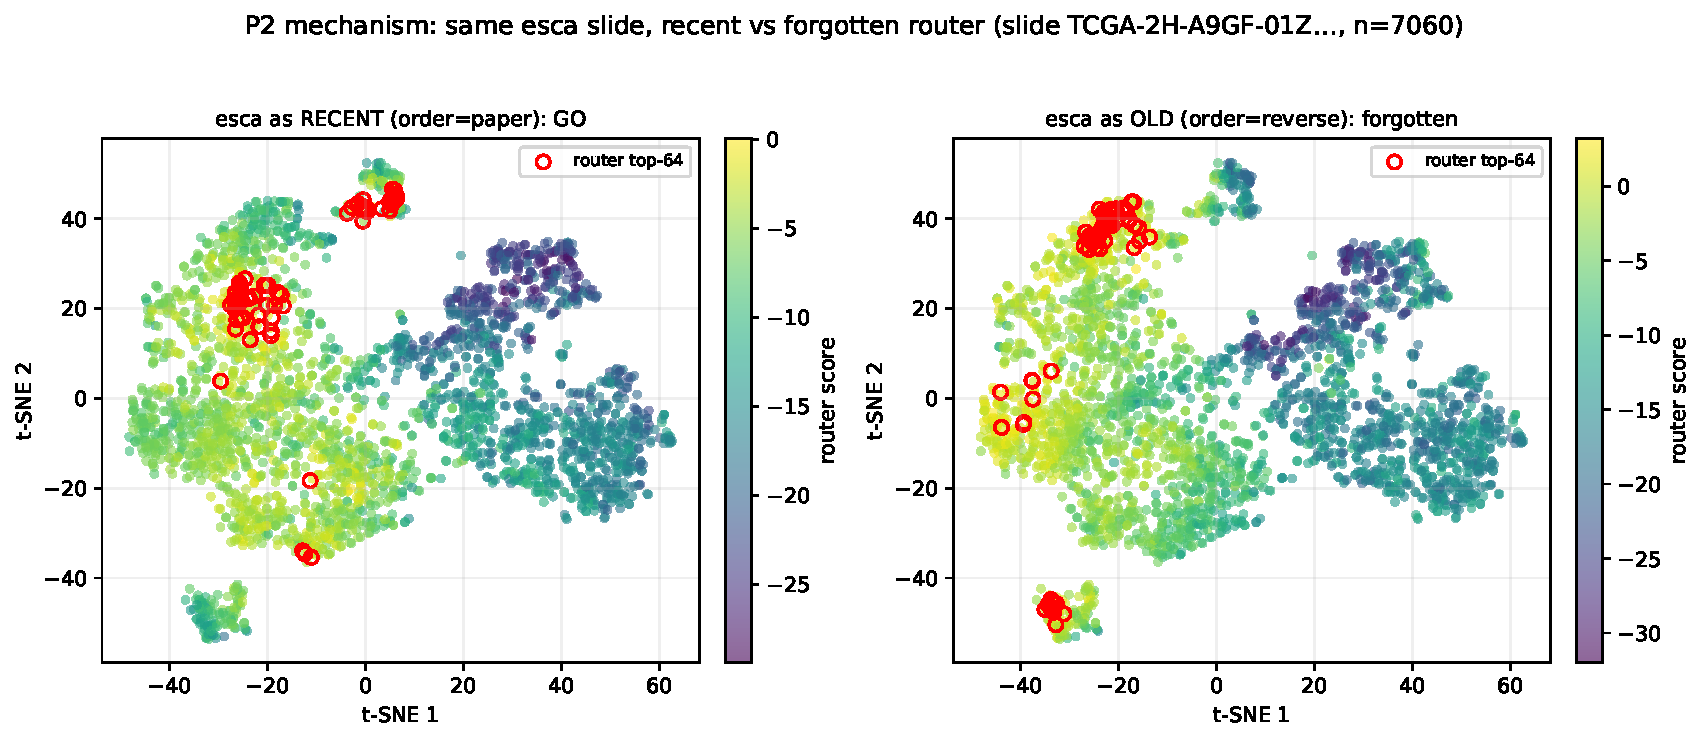
\includegraphics[width=0.66\linewidth]{P2contrast_esca_fold1.pdf}
\caption{\textbf{Mechanism.} The same esca slide in CONCH feature space
(shared t-SNE). Recent router (left) scores and selects the
diagnostically relevant cluster; forgotten router (right) keeps
structured scores but concentrates its top-$K$ on a
later-task-salient subpopulation---confident mis-prioritization.}
\label{fig:mechanism}
\end{figure}

The forgotten router does not become noise; it confidently
mis-prioritizes (Fig.~\ref{fig:mechanism}), explaining sub-random
behavior.

\subsection{Mitigation: NSM Recovers, EWC Does Not}
\label{sec:mitigation}

\begin{table}[htbp]
\centering
\caption{Mitigation ablation (esca oldest task, reverse order, mean 3 folds).
NSM (ours) fully recovers old-task selection; EWC and zero-shot fall
short. ``best base'' = best heuristic@64 (the bar to clear).}
\label{tab:mitigation}
\small\begin{tabular}{lcccccccc}
\toprule
Strategy & @256 & @128 & @64 & @32 & best base@64 & mACC & Fgt. & \go/\nogo \\
\midrule
Naive continual  & 0.511 & 0.400 & \textbf{0.333} & 0.333 & 0.822 & 0.595 & 0.454 & \nogo\,(0/3) \\
EWC-on-router    & 0.622 & 0.422 & \textbf{0.400} & 0.267 & 0.822 & ---   & ---   & \nogo\,(0/3) \\
Zero-shot nav.~\cite{zeroslide}
                 & ---   & ---   & ---            & ---   & ---   & 0.858 & \textbf{0.000} & --- \\
\textbf{NSM (ours)}
                 & 0.933 & 0.933 & \textbf{0.933} & 0.933 & 0.822 & \textbf{0.935} & \textbf{0.000} & \go\,(3/3) \\
\midrule
LoRA-NSM (planned) & --- & --- & --- & --- & --- & TBD & TBD & --- \\
\bottomrule
\end{tabular}
\end{table}

NSM restores esca@64 from $0.333$ to $\mathbf{0.933}$ (Table~\ref{tab:mitigation}):
flat across all budgets, above every heuristic (3/3 folds). The
zero-shot navigator achieves mACC $0.858$ without any training---a
strong training-free ceiling that NSM surpasses by $+7.7$\,pp via
task-specific learned routing. EWC barely moves the needle ($0.400$;
0/3): weight-level consolidation is insufficient for a selection
policy (Sec.~\ref{sec:discussion}).

\subsection{Sequential Observation: $\lambda$ Sweep}
\label{sec:lambda}

We run the SBO on the trained NSM skill bank (fold 1, reverse order,
all 4 tasks) sweeping $\lambda\in\{0,1,2,4\}$, \texttt{normalize\_base=True},
\texttt{redundancy\_mode=maxsim}, $K{=}64$, $k_\text{step}{=}16$.

\begin{table}[htbp]
\centering
\caption{SBO $\lambda$ sweep: sequential (nsm\_seq) vs.\ one-shot
(nsm\_oneshot) accuracy at $K{=}64$ (fold 1, reverse order).
$\lambda{=}0$ confirms seq$\equiv$oneshot (baseline). Optimal
$\lambda{=}0.5$--$1.0$ causes negligible accuracy loss while making
selection genuinely adaptive. Large $\lambda$ forces the agent off
spatially-clustered diagnostic regions, degrading accuracy.}
\label{tab:lambda}
\small\begin{tabular}{lccccccccc}
\toprule
$\lambda$ & \multicolumn{2}{c}{esca} & \multicolumn{2}{c}{rcc} & \multicolumn{2}{c}{brca} & \multicolumn{2}{c}{lung} \\
 & seq & 1shot & seq & 1shot & seq & 1shot & seq & 1shot \\
\midrule
0.0 & 0.867 & 0.867 & 0.961 & 0.961 & 0.860 & 0.860 & 0.810 & 0.810 \\
1.0 & 0.867 & 0.867 & 0.961 & 0.961 & 0.860 & 0.860 & 0.800 & 0.810 \\
2.0 & 0.800 & 0.867 & 0.961 & 0.961 & 0.850 & 0.860 & 0.768 & 0.810 \\
4.0 & 0.267 & 0.867 & 0.355 & 0.961 & 0.570 & 0.860 & 0.684 & 0.810 \\
\bottomrule
\end{tabular}
\end{table}

\noindent\textbf{Key findings.} (1) $\lambda{=}0$ confirms seq$\equiv$oneshot
(mechanism baseline). (2) $\lambda{=}1$--$2$: seq diverges from
one-shot with minimal accuracy cost---the SBO is genuinely
sequential. (3) Large $\lambda$: WSI tumor patches are spatially
clustered, and the router has learned these clusters; MMR with large
$\lambda$ forces exploration of non-diagnostic regions, degrading
accuracy. The optimal $\lambda{=}0.5$--$1.0$ respects learned spatial
priors while providing coverage diversity.

\FloatBarrier
% =====================================================================
\section{Discussion}
\label{sec:discussion}

\noindent\textbf{Selection forgetting is distinct from classifier forgetting.}
With the backbone frozen, every old-task degradation is attributable to
the selection module---a forgetting phenomenon that the
continual-learning literature, focused on classifier/representation,
does not capture. This matters broadly for budget-constrained inference
with frozen FMs, where a learned selector front-ends a fixed predictor.

\noindent\textbf{Why EWC fails while NSM fully recovers.}
Per-task recovery ($0.33\to0.93$) shows the selection signal is still
present in the frozen features. EWC penalizes drift of individual
weights, but what matters is the induced \emph{ordering} of patch
scores---a global, nonlinear function of those weights. More promising
are: (a)~distilling old-task patch score rankings (pairwise/listwise),
(b)~function-space regularization over orderings, or (c)~LoRA-NSM.

\noindent\textbf{SBO and spatial geometry of diagnostic regions.}
The $\lambda$ sweep reveals that tumor patches cluster spatially and
the router has encoded this geometry. Pure MMR-diversity (large
$\lambda$) disrupts the learned spatial prior; the ideal SBO should
respect it. Promising extensions: adaptive $\lambda$ (decrease once
the high-confidence cluster is seen), or RL-based sequential policy.

\noindent\textbf{LoRA-NSM: scalable navigation skill memory.}
\label{sec:lora}
Per-task NSM grows $O(T\!\times\!533\text{KB})$. LoRA-NSM (rank $r{=}4$
on each router linear layer) stores $\approx4$KB/task---a ${\sim}130\times$
reduction---while sharing a frozen router base across tasks. This is
the N7 experiment target (7/20).

\noindent\textbf{Limitations.}
(i)~Four TCGA cohorts; longer sequences and multi-site data needed.
(ii)~Oracle context gate; task-free gating is an open problem.
(iii)~$\lambda$ sweep: fold~1 only; 3-fold confirmation is future work.
(iv)~Static SBO; learned sequential policy (RL-based) may better
exploit multi-step structure.

% =====================================================================
\section{Conclusion}
\label{sec:conclusion}
We identify \textbf{selection forgetting}---a new failure mode where a
trainable patch router in frozen-FM continual WSI classification
forgets how to navigate for old tasks, falling below random. The CNL
framework addresses this: the MicroRouter learns task-specific
navigation skills; the SBO makes observation genuinely adaptive via
MMR redundancy; and NSM stores per-task routing policies, recovering
mACC from $0.595$ to $\mathbf{0.935}$ with zero forgetting. The
$\lambda$ sweep reveals that optimal multi-step selection respects
the spatial clustering of diagnostic regions. LoRA-NSM (${\sim}4$KB/task,
${\sim}130\times$ smaller) is identified as the clear scalable next step.

\FloatBarrier
\bibliographystyle{splncs04}
\bibliography{references}

\end{document}
